Let
%\label{constr/7prob:tri_polar}
\begin{align}
\vec{A} = c\myvec{\cos \theta\\  \sin \theta} ,\vec{B} = \myvec{0\\0},\vec{C} = \myvec{a\\0},
\end{align}
Using the cosine formula in  $\triangle ABC$, 
\begin{align}
b^2 = a^2 + c^2 - 2ac \cos B 
\\
\implies (c+b)(c-b) + 8^2 - 2 \times 8\times \brak{\frac{1}{\sqrt{2}}}c = 0 
\\
\implies (7 - 16\sqrt{2})c + 7b = -128
\end{align}
upon simplification.  From the given information,
\begin{align}
% \implies c - b = 3.5
% \\
c - b =\frac{7}{2},
\end{align}
and teh above equations  can be expressed as the matrix equation
\begin{align}
\myvec{7 - 16\sqrt{2} & 7\\1 & -1}\myvec{c\\b} = \myvec{-128 \\ \frac{7}{2}}
\end{align}
yielding
\begin{align}
\myvec{c\\b}=\myvec{11.99\\8.49}
\end{align}
Thus, the vertices of $\triangle ABC$ are
\begin{align}
\vec{A} = 11.99\myvec{\cos45\\\sin45} , \vec{B} = \myvec{0\\0},\vec{C} = \myvec{8\\0}.
\end{align}
which are used to plot Fig.    \ref{constr/7/fig:LMN}.
\begin{figure}[!ht]
    \centering
    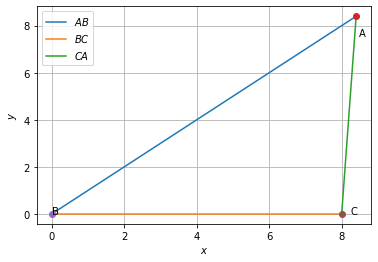
\includegraphics[width=\columnwidth]{solutions/7/Fig1.png}
    \caption{$\triangle ABC$}
    \label{constr/7/fig:LMN}
\end{figure}

 
 
 